\documentclass[10pt]{exam-zh}
\title{2025—2026 学年度上学期\\ 高一学期末考试数学试卷}
\begin{document}
\maketitle


%\section{选择题：本题共 8 小题，每小题 5 分，共 40 分.在每小题给出的四个选项中，只有一项是符合题目要求的.}
%
%\begin{question}
%    已知集合 \( A = \{ x \mid 0 < x < 3 \} \)，\( B = \{-1,0,1,2,3\} \)，则 \( A \cap B = \)
%    \begin{choices}
%        \item \( \{1,2\} \)
%        \item \( \{0,1,2\} \)
%        \item \( \{-1,0,1,2\} \)
%        \item \( \{-2,-1,0,1,2\} \)
%    \end{choices}
%\end{question}
%
%\begin{question}
%已知函数 \( f(x) = (m^2 + m - 1)x^{m^2 - 2} \) 是幂函数，且在 \( (0,+\infty) \) 上递增，则实数 \( m = \)
%    \begin{choices}
%        \item \( 2 \)
%        \item \( -2 \)
%        \item \( 1 \)
%        \item \( 1 \) 或 \( -2 \)
%    \end{choices}
%\end{question}
%
%\begin{question}
%命题“\( \exists x \in \mathbf{R} \)，\( x^2 - x + 3 \leq 0 \)”的否定是
%    \begin{choices}
%        \item \( \exists x \in \mathbf{R} \)，\( x^2 - x + 3 \geq 0 \)
%        \item \( \exists x \in \mathbf{R} \)，\( x^2 - x + 3 > 0 \)
%        \item \( \forall x \in \mathbf{R} \)，\( x^2 - x + 3 \leq 0 \)
%        \item \( \forall x \in \mathbf{R} \)，\( x^2 - x + 3 > 0 \)
%    \end{choices}
%\end{question}
%
%\begin{question}    
%已知函数 \( f(x) = \begin{cases} x + 1, & x < 3 \\ f(x - 3), & x \geq 3 \end{cases} \)，则 \( f(7) = \)
%    \begin{choices}
%        \item \( 16 \)
%        \item \( 8 \)
%        \item \( 2 \)
%        \item \( -2 \)
%    \end{choices}
%\end{question}
%    
%\begin{question}
%函数 \( f(x) = 2^{|x + 1|} \) 的图象大致为
%%    \begin{choices}
%%        \item 选项 A（图象：关于 \( x = -1 \) 对称，\( x = -1 \) 时 \( y = 1 \)，\( x > -1 \) 时递增）
%%        \item 选项 B（图象：关于 \( x = -1 \) 对称，\( x = -1 \) 时 \( y = 1 \)，\( x > -1 \) 时递减）
%%        \item 选项 C（图象：关于 \( x = 1 \) 对称，\( x = 1 \) 时 \( y = 1 \)，\( x > 1 \) 时递减）
%%        \item 选项 D（图象：关于 \( x = -1 \) 对称，\( x = -1 \) 时 \( y = 1 \)，\( x > -1 \) 时递增且增长更快）
%%    \end{choices}
%	\begin{center}
%	
\includegraphics[width=\linewidth]{1-5.png}
%	\end{center}
%\end{question}
%
%\begin{question}
%使得不等式 \( 2^m > 2^n \) 成立的一个充分不必要条件是
%    \begin{choices}
%        \item \( \dfrac{1}{n} > \dfrac{1}{m} \)
%        \item \( \sqrt{m} > \sqrt{n} \)
%        \item \( m^2 > n^2 \)
%        \item \( m^3 > n^3 \)
%    \end{choices}
%\end{question}
%
%\begin{question}
%已知函数 \( f(x) = \begin{cases} (4a - 1) \cdot 2^x, & x < 1 \\ x^2 - ax + 6, & x \geq 1 \end{cases} \) 是 \( \mathbf{R} \) 上的单调递增函数，则实数 \( a \) 的取值范围是
%    \begin{choices}
%        \item \( \left( \dfrac{1}{4}, 1 \right] \)
%        \item \( \left( \dfrac{1}{4}, 2 \right] \)
%        \item \( [2, +\infty) \)
%        \item \( [1, 2] \)
%    \end{choices}
%\end{question}
%
%\begin{question}
%已知函数 \( f(x) = x^2 + 2x + m(e^{x + 1} + e^{-x - 1}) \) 的图象与 \( x \) 轴有且只有一个交点，则 \( m \) 的值为
%    \begin{choices}
%        \item \( -\dfrac{1}{2} \)
%        \item \( \dfrac{1}{3} \)
%        \item \( \dfrac{1}{2} \)
%        \item \( 1 \)
%    \end{choices}
%\end{question}
%
%\section{选择题：本题共 3 小题，每小题 6 分，共 18 分.在每小题给出的选项中，有多项符合题目要求.全部选对的得 6 分，部分选对的得部分分，有选错的得 0 分.}
%
%\begin{question}
%下列各选项给出的数学命题中，正确的是
%    \begin{choices}
%        \item 集合 \( A = \{ x \mid y = \sqrt{x^2 + 1} \} \)，\( B = \{ y \mid y = \sqrt{x^2 + 1} \} \) 表示相等集合
%        \item 若 \( y = f(x) \) 是一次函数，满足 \( f(f(x)) = x + 2 \)，则 \( f(x) = x + 1 \)
%        \item 函数 \( y = \dfrac{x - 2}{x + 1} (x \geq 1) \) 的值域为 \( \left[ -\dfrac{1}{2}, 1 \right) \)
%        \item 若关于 \( x \) 的不等式 \( ax^2 + bx + c > 0 \) 的解集为 \( (-2, 3) \)，则不等式 \( cx^2 - bx + a < 0 \) 的解集为 \( \left( -\dfrac{1}{3}, \dfrac{1}{2} \right) \)
%    \end{choices}
%\end{question}
%    
%\begin{question}
%已知 \( a > 0, b > 0 \)，且 \( \dfrac{1}{a} + \dfrac{4}{b} = 4 \)，则
%    \begin{choices}
%        \item \( b > 1 \)
%        \item \( a + b \geq \dfrac{9}{4} \)
%        \item \( ab \leq 1 \)
%        \item \( \dfrac{1}{a^2} + \dfrac{16}{b^2} \geq 8 \)
%    \end{choices}
%\end{question}
%    
%\begin{question}
%已知定义域为 \( \mathbf{R} \) 的函数 \( f(x) \)，对任意实数 \( x, y \) 都有 \( f(x + y) + f(x - y) = f(x)f(y) \)，且 \( f(2) = -2 \)，则以下结论一定正确的有
%    \begin{choices}
%        \item \( f(0) = 1 \)
%        \item \( f(x) \) 是奇函数
%        \item \( f(x) \) 关于点 \( (1, 0) \) 中心对称
%        \item \( f(1) + f(2) + \cdots + f(2025) = 0 \)
%    \end{choices}
%\end{question}    
%\begin{center}
%\vspace{0.5cm}
%\Large
%\textbf{第Ⅱ卷}
%\vspace{0.5cm}
%\end{center}
%
%\section{填空题：本题共 3 小题，每小题 5 分，共 15 分.}
%
%\begin{question}
%    计算 \( 8^{\dfrac{2}{3}} + 2\lg 2 + \lg 25 = \) \(\underline{\quad\quad\quad\quad\quad}\)
%\end{question}    
%
%    
%\begin{question}
%已知函数 \( f(x) = \begin{cases} x + 2, & x < 0 \\ x^2 - 2x + 2, & x \geq 0 \end{cases} \)，若当 \( x \in [a, b] \) 时，\( 1 \leq f(x) \leq 10 \)，则 \( b - a \) 的最大值是 \(\underline{\quad\quad\quad\quad\quad}\)
%\end{question}    
%
%\begin{question}
%已知函数 \( f(x) = ax^2 - bx - a + b \)，\( x \in [0, m] \)，对任意 \( 2b \geq a > 0 \)，不等式 \( f(x) \leq (2b - a)(x + 1) \) 恒成立，则 \( m \) 的最大值为 \(\underline{\quad\quad\quad\quad\quad}\)
%\end{question}    
%
%
%\section{解答题：本题共 5 小题，共 77 分.解答应写出文字说明、证明过程或演算步骤.}
%
%\begin{problem}
%    (13 分) 设 \( U = \mathbf{R} \)，\( A = \{ x \mid 2 < x < 4 \} \)，\( B = \{ x \mid x^2 - 4x + a \leq 0, a \in \mathbf{R} \} \).
%    \begin{enumerate}
%        \item 当 \( a = 3 \) 时，求 \( A \cap B \)，\( (\complement_U A) \cup B \)；
%        \item 若 \( A \cap B = A \)，求实数 \( a \) 的取值范围.
%    \end{enumerate}
%\end{problem}
%\begin{problem}
%    (15 分) 已知函数 \( f(x) = (a^2 - 2a - 2)a^x (a > 0 \text{ 且 } a \neq 1) \) 过点 \( (0, 1) \).
%    \begin{enumerate}
%        \item 求 \( a \) 的值，并写出 \( f(x) \) 的解析式；
%        \item 判断 \( F(x) = f(x) - \dfrac{1}{f(x)} \) 的奇偶性，并用定义证明；
%        \item 若 \( f(x) = h(x) + t(x) \)，且 \( h(x) \) 为奇函数，\( t(x) \) 为偶函数，写出 \( h(x) \) 的解析式（无需证明）.
%    \end{enumerate}
%\end{problem}
%
%\begin{problem}
%(15 分) 为加快落实新旧动能转换，某单位在国家科研部门的支持下，进行技术攻关，新上了一个项目，该项目可以把二氧化碳处理转化为一种可利用的化工产品.经测算，该项目月处理成本 \( y \)（元）与月处理量 \( x \)（吨）之间的函数关系可近似地表示为 \( y = \begin{cases} \dfrac{1}{3}x^3 - 80x^2 + 5040x, & x \in [120, 144) \\ \dfrac{1}{2}x^2 - 200x + 80000, & x \in [144, 500] \end{cases} \)，且每处理一吨二氧化碳得到可利用的化工产品价值为 200 元，若该项目不盈利，国家将给予补偿.
%    \begin{enumerate}
%        \item 当 \( x \in [200, 300] \) 时，判断该项目能否盈利.如果盈利，求出最大利润；如果该项目不盈利，要使该单位不亏损，则国家需要补偿资金的范围是多少元？
%        \item 该项目每月处理量为多少吨时，才能使每吨的平均处理成本最低？
%    \end{enumerate}
%\end{problem}    
%\begin{problem}
%    (17 分) 已知函数 \( f(x) = \dfrac{ax + b}{x^2 + 1} \)，若 \( f(1) = \dfrac{1}{2} \)，且当 \( x \neq 0 \) 时 \( f(x) = f\left( \dfrac{1}{x} \right) \).
%    \begin{enumerate}
%        \item 求 \( a, b \) 的值，并写出 \( f(x) \) 的解析式；
%        \item 判断函数 \( f(x) \) 在 \( [1, +\infty) \) 上的单调性，并用定义证明；
%        \item 若对任意的 \( x \in \left[ \dfrac{1}{3}, \dfrac{3}{4} \right] \) 都有 \( f(x) + f(3x - a) \leq 0 \) 恒成立，求实数 \( a \) 的取值范围.
%    \end{enumerate}
%\end{problem}
%
%\begin{problem}
%    (17 分) 俄国数学家切比雪夫（1821—1894）是研究直线逼近函数的理论先驱. 设 \( f(x) \) 是定义在 \( [m, n] \) 上的连续函数，称 \( E = \max\limits_{m \leq x \leq n} |f(x) - (ax + b)| \) 为 \( f(x) \) 与直线 \( g(x) = ax + b \) 的偏差. 若存在 \( x_0 \in [m, n] \) 使得 \( |f(x_0) - g(x_0)| = E \)，则称 \( x_0 \) 为直线 \( g(x) \) 的偏差点. 记 \( A = \{ g(x) = ax + b \mid a, b \in \mathbf{R} \} \)，若存在 \( g_0(x) \in A \) 使得 \( \max\limits_{m \leq x \leq n} |f(x) - g_0(x)| = \min\limits_{a, b \in \mathbf{R}} \max\limits_{m \leq x \leq n} |f(x) - g(x)| \) 则称 \( g_0(x) \) 为 \( f(x) \) 在切比雪夫意义下的最佳逼近直线.
%    \begin{enumerate}
%        \item 函数 \( f(x) = x^2, x \in [-1, 2] \)，\( g(x) = x + 1 \)，求 \( f(x), g(x) \) 的偏差以及偏差点；
%        \item 函数 \( f(x) = 3x + \dfrac{4}{x}, x \in [1, 4], g(x) = 2x + b \)，求 \( f(x), g(x) \) 的偏差的最小值，并求出取得最小值时 \( b \) 的值；
%        \item 证明：直线 \( g(x) = \dfrac{1}{2}x + \dfrac{1}{4} \) 是函数 \( f(x) = \sqrt{x} \) 在 \( x \in [0, 4] \) 上的最佳逼近直线.
%    \end{enumerate}
%\end{problem}




	\begin{center}
	\large	\textbf{第I卷（选择题，共58分）}
	\end{center}
	
	
	\section{单选题：共8小题，每小题5分，共40分。在每小题给出的四个选项中，只有一项是符合题目要求的。}
	
	\begin{enumerate}[leftmargin=*, label=\arabic*.]
		\item 已知全集 \( U = \{-2, -1, 0, 1, 2, 3\} \)，\( A = \{x \in \mathbb{N} \mid 0 \leq x \leq 3\} \)，则 \( C_U A = \)\paren
		\begin{choices}[label=\Alph*.]
			\item \(\{-2, -1\}\)
			\item \(\{-2, -1, 0\}\)
			\item \(\{0, 1, 2, 3\}\)
			\item \(\{1, 2, 3\}\)
		\end{choices}
		
		\item 设 \( x \in \mathbb{R} \)，则“\( x(2 + x) > 0 \)”是“\( 0 < x < 1 \)”的\paren
		\begin{choices}[label=\Alph*.]
			\item 充分不必要条件
			\item 必要不充分条件
			\item 充要条件
			\item 既不充分也不必要条件
		\end{choices}
		
		\item 已知 \(\tan(\pi + \theta) = -3\)，则 \(\dfrac{3\sin\theta - \cos\theta}{\sin\theta + 5\cos\theta} = \)\paren
		\begin{choices}[label=\Alph*.]
			\item 5
			\item $-5$
			\item 1
			\item $-1$
		\end{choices}
		
		\item 函数 \( y = \ln(x^2 - 3x + 2) \) 的单调递减区间是\paren
		\begin{choices}[label=\Alph*.]
			\item \((-\infty, 1)\)
			\item \(\left(\dfrac{3}{2}, +\infty\right)\)
			\item \(\left(-\infty, \dfrac{3}{2}\right)\)
			\item \((2, +\infty)\)
		\end{choices}
		
		\item 已知 \(\cos\left(\alpha + \dfrac{\pi}{12}\right) = \dfrac{2}{3}\)，则 \(\sin\left(2\alpha - \dfrac{\pi}{3}\right) = \)\paren
		\begin{choices}[label=\Alph*.]
			\item \(-\dfrac{1}{9}\)
			\item \(\dfrac{1}{9}\)
			\item \(-\dfrac{7}{9}\)
			\item \(\dfrac{7}{9}\)
		\end{choices}
		
		\item 已知函数 \( f(x) \) 是定义在 \([b-2, 3]\) 上的偶函数，且 \( f(x) \) 在 \([0, 3]\) 上单调递减，若 \( f(x+b) > f(2) \)，则 \( x \) 的取值范围是\paren
		\begin{choices}[label=\Alph*.]
			\item \((-1, 3)\)
			\item \((-3, 1)\)
			\item \((-4, 2)\)
			\item \((-2, 4)\)
		\end{choices}
		
		\item 若函数 \( f(x) = 
		\begin{cases} 
			ax + 3, & x \leq 0 \\ 
			\log_{\dfrac{1}{3}}(x+1) + a, & x > 0 
		\end{cases} \) 存在最大值，则实数 \( a \) 的取值范围是\paren
		\begin{choices}[label=\Alph*.]
			\item (0, 4)
			\item [0, 4]
			\item (0, 3)
			\item [0, 3]
		\end{choices}
		
		\item 已知函数 \( f(x) = \sin\left(\omega x + \dfrac{\pi}{3}\right)(\omega > 0) \) 在 \(\left(0, \dfrac{\pi}{3}\right)\) 上存在零点，且在 \(\left(\dfrac{2\pi}{3}, \pi\right)\) 上单调递增，则 \(\omega\) 的取值范围为\paren
		\begin{choices}[label=\Alph*.]
			\item (2,3]
			\item \(\left(2,\dfrac{13}{6}\right]\)
			\item \(\left[\dfrac{7}{4}, \dfrac{13}{6}\right]\)
			\item \(\left[\dfrac{7}{4}, 3\right]\)
		\end{choices}
	\end{enumerate}
	
	\section{多选题：共 3 小题，每小题 6 分，共 18 分。在每小题给出的选项中，有多项符合题目要求，全部选对的得 6 分，部分选对的得部分分，有选错的得 0 分。}
	
	\begin{enumerate}[leftmargin=*, label=\arabic*.]
		\item[9.] 已知函数 \( y = a^{x-2} + 1 \) (\(a > 0\) 且 \(a \neq 1\)) 过定点 \((p,q)\)，若正实数 \(m,n\) 满足 \(m+n= pq\)，则下列说法正确的是\paren
		\begin{choices}[label=\Alph*.]
			\item \( mn \) 的最大值为 4
			\item \( m^2 + n^2 \) 的最大值为 8
			\item \(\dfrac{1}{m} + \dfrac{4}{n}\) 的最小值为 \(\dfrac{9}{4}\)
			\item \( m^2 + 2n \) 的最小值为 8
		\end{choices}
		
		\item[10.] 已知函数 \( f(x) = A\sin(\omega x + \varphi)(A>0,\omega>0, \left|\varphi\right|\le\dfrac{\pi}{2} )\) 的部分图象如图所示，则\paren\\
		\begin{minipage}{0.7\linewidth}
			\begin{choices}[label=\Alph*.]
				\item \(\varphi = \dfrac{\pi}{6}\)
				\item 函数 \( f(x) \) 在区间 \((-\dfrac{\pi}{3}, \dfrac{\pi}{3})\) 上不单调
				\item 若 \( x \in [-\dfrac{\pi}{2}, \dfrac{\pi}{12}] \)，则函数 \( f(x) \) 的值域是 \([-1, \sqrt{3}]\)
				\item \( y = 2\cos\left(2x - \dfrac{5\pi}{6}\right) \) 图象可以由 \( y = f(x) \) 图象向右平移 \(\dfrac{\pi}{4}\) 个单位长度得到
			\end{choices}
		\end{minipage}
		\begin{minipage}{0.3\linewidth}
			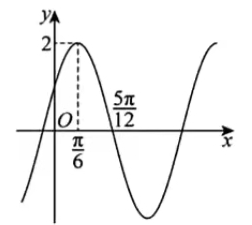
\includegraphics[width=\linewidth]{f1.png}
		\end{minipage}

		
		\item[11.] 已知对 \(\forall x,y \in \mathbb{R}\)，\( f(x+y)+f(x-y)=f(x)f(y) \)，\( f(1)=1 \) 则下列说法中正确的是\paren
		\begin{choices}[label=\Alph*.]
			\item \( f(0)=2 \)
			\item \( y=f(x) \) 可以为一次函数
			\item \( f(x)+f(x+3)=0 \)
			\item \( f(1)+f(2)+\cdots+f(2025)=-2 \)
		\end{choices}
	\end{enumerate}
	

	\begin{center}
		\large	\textbf{第II卷（非选择题，共 92 分）}
	\end{center}
	\section{填空题：本大题共 3 小题，每小题 5 分，共 15 分。将答案填在答题卡相应的位置上。}
	
	\begin{enumerate}[leftmargin=*, label=\arabic*.]
		\item[12.] 已知角 \(\theta\) 的终边经过点 \( P(1,-2) \)，则 \(\tan 2\theta = \underline{\qquad\qquad}\)。
		
		\item[13.] \( e^{\ln 3} - \log_2 3 \cdot \log_3 4 + 8^{\dfrac{2}{3}} = \underline{\qquad\qquad}\)。
		
		\item[14.] 已知函数 \( f(x) = |x^2 + ax + 1| (a \in \mathbb{R}) \) 的图象与直线 \( y = 2x \) 有两个交点，与直线 \( y = 2 \) 有四个交点，则 \( a \) 的取值范围是 \(\underline{\qquad\qquad}\)。
	\end{enumerate}
	
	\section{解答题：本大题共 5 小题，共 77 分。解答应写出文字说明，证明过程或演算步骤。}
	
	\begin{enumerate}[leftmargin=*, label=\arabic*.]
		\item[15.] （13 分）\\
		已知角 \(\alpha, \beta \in \left(0, \dfrac{\pi}{2}\right)\) 且 \(\cos \alpha = \dfrac{\sqrt{5}}{5}\)。
		\begin{enumerate}[label=(\arabic*)]
			\item 若 \(\tan \beta = \dfrac{1}{3}\)，求 \(\alpha - \beta\) 的值；
			\item 若 \(\sin(\beta - \alpha) = \dfrac{7}{25}\)，求 \(\sin(\alpha + \beta)\) 的值。
		\end{enumerate}
		\newpage
		\item[16.] （15 分）\\
		已知函数 \(f(x) = 2\sin^2 x + \cos\left(2x - \dfrac{\pi}{3}\right) - 1\)。
		\begin{enumerate}[label=(\arabic*)]
			\item 求函数 \(f(x)\) 的最小正周期和单调递增区间；
			\item 当 \(x \in \left[-\dfrac{\pi}{4}, \dfrac{\pi}{4}\right]\) 时，求函数 \(f(x)\) 的值域。
		\end{enumerate}
			\vspace{8cm}
		\item[17.] （15 分）\\
		已知函数 \(f(x) = 9^x - a \cdot 3^x + 1 (a \in \mathbb{R})\)。
		\begin{enumerate}[label=(\arabic*)]
			\item 当 \(a = 2\) 时，求函数 \(f(x)\) 在 \(x \in [-1, 1]\) 上的值域；
			\item 设 \(g(x) = \cos x\)。若对 \(\forall x_1 \in \left[\dfrac{\pi}{2}, \dfrac{2\pi}{3}\right], \forall x_2 \in [1, 2]\) 都有 \(g(x_1) < f(\log_3 x_2)\) 成立，求 \(a\) 的取值范围。
		\end{enumerate}
		\newpage
		\item[18.] （17 分）\\
		已知函数 \( f(x) = \ln \dfrac{4^x + b}{2^x} \) 为偶函数，\( g(x) = \ln (m \cdot 2^x - 2m) \)。
		\begin{enumerate}[label=(\arabic*)]
			\item 求实数 \( b \) 的值，并判断 \( f(x) \) 在 \( (0, +\infty) \) 上的单调性（无需证明）；
			\item 当 \( x \in (0, 1) \) 时，\( f(2x+1) < f(x+a) \) 恒成立，求实数 \( a \) 的取值范围；
			\item 当 \( x \in [1, 2] \) 时，\( f(x) \geq g(x) \) 恒成立，求实数 \( m \) 的取值范围。
		\end{enumerate}
		\vspace{8cm}
		\newpage
		\item[19.] （17 分）\\
		已知函数 \( f(x) = \sin(\omega x + \varphi) \)（\(\omega \in (1, 3)\)，\(|\varphi| < \dfrac{\pi}{2}\)），\(\forall x \in \mathbb{R}\)，\(f(x+2\pi) = f(x) + f(2\pi)\) 恒成立。
		\begin{enumerate}[label=(\arabic*)]
			\item 求 \( f(0) \) 的值及 \( f(x) \) 的解析式；
			\item \( g(x) = \log_2(-x^2 + x + a) \)，当 \( x \in (0, \dfrac{\pi}{4}) \) 时，\( y = g\left(f(x)\right) \) 有两个零点 \( x_1, x_2 \)，求 \( a \) 的取值范围；
			\item 已知 \( a, b, c \in (0, A) \)，且以 \( a, b, c \) 为边能够组成三角形，对于任意满足上述条件的 \( a, b, c \)，若以 \( f(\dfrac{a}{2}), f(\dfrac{b}{2}), f(\dfrac{c}{2}) \) 为边也能够组成三角形，求 \( A \) 的最大值。
		\end{enumerate}
	\end{enumerate}
\small
\begin{enumerate}
	\item  由题设对一切 $x\in\mathbb{R}$ 有\( \sin\bigl(\omega(x+2\pi)+\varphi\bigr)=\sin(\omega x+\varphi)+\sin(2\pi\omega+\varphi).\)
令 $t=\omega x+\varphi$，则 \( \sin(t+2\pi\omega)=\sin t\cos(2\pi\omega)+\cos t\sin(2\pi\omega).\)
代入并整理得
\[
\bigl(\cos(2\pi\omega)-1\bigr)\sin t+\sin(2\pi\omega)\cos t\equiv \sin(2\pi\omega+\varphi).
\]

左端关于 $t$ 为正弦余弦的线性组合，要对所有 $t$ 恒为常数，只能有
\(\cos(2\pi\omega)-1=0,\sin(2\pi\omega)=0.\)

故 $2\pi\omega=2k\pi\,(k\in\mathbb{Z})$，即 $\omega=k$。结合 $\omega\in(1,3)$ 得 $\omega=2$。
此时原恒等式化为 $f(x+2\pi)=f(x)+f(2\pi)$，但又有 $f(x+2\pi)=f(x)$（周期性），故 $f(2\pi)=0$。
而 $f(2\pi)=\sin(4\pi+\varphi)=\sin\varphi$，且 $|\varphi|<\dfrac{\pi}{2}$，故 $\varphi=0$。
因此
\(
f(0)=0, f(x)=\sin 2x.
\)

\item  令 $u=f(x)=\sin 2x$。当 $x\in\left(0,\dfrac{\pi}{4}\right)$ 时，$2x\in\left(0,\dfrac{\pi}{2}\right)$，故 $u\in(0,1)$ 且随 $x$ 严格递增。
函数 $y=g(u)=\log_2(-u^2+u+a)$ 的零点满足
\[
\log_2(-u^2+u+a)=0\iff -u^2+u+a=1\iff u^2-u+(1-a)=0.
\]
要在 $u\in(0,1)$ 内有两个不同实根（从而对应 $x\in\left(0,\dfrac{\pi}{4}\right)$ 内两个不同零点），需
\[
\Delta=1-4(1-a)=4a-3>0\iff a>\dfrac{3}{4},
\]
且两根
\(
u_{1,2}=\dfrac{1\pm\sqrt{4a-3}}{2}
\)
都落在 $(0,1)$。由 $u_2<1\iff \sqrt{4a-3}<1\iff a<1$（同时也保证 $u_1>0$）。
综上
\(
a\in\left(\dfrac{3}{4},\,1\right).
\)

\item  此时 $f\!\left(\dfrac{a}{2}\right)=\sin a$，同理得到三边为 $\sin a,\sin b,\sin c$。

\textbf{必要性：} 若 $A>\dfrac{5\pi}{6}$，取 $a=\dfrac{\pi}{2}$，$b=c=A-\varepsilon$（$\varepsilon>0$ 足够小），则 $a,b,c\in(0,A)$ 且 $b+c>\pi/2$，$a+b>c$，$a+c>b$，所以 $a,b,c$ 能组成三角形。
但当 $A>\dfrac{5\pi}{6}$ 时，$\sin(A-\varepsilon)<\dfrac{1}{2}$（取 $\varepsilon$ 足够小即可），从而
\(
\sin b+\sin c=2\sin(A-\varepsilon)<1=\sin\dfrac{\pi}{2}=\sin a,
\)
于是 $\sin a,\sin b,\sin c$ 不能组成三角形，矛盾。故 $A\le \dfrac{5\pi}{6}$。

\textbf{充分性：} 当 $A\le\dfrac{5\pi}{6}$ 时，对任意 $a,b,c\in(0,A)$ 能组成三角形。
若其中存在一边 $\ge\dfrac{\pi}{2}$，则另外两边之和 $>\dfrac{\pi}{2}$，从而至少一边 $>\dfrac{\pi}{4}$，于是两条对应正弦边之和严格大于 $1$，而任意正弦边均小于等于 $1$，三角不等式成立。
若三边都 $<\dfrac{\pi}{2}$，则 $\sin x$ 在 $(0,\dfrac{\pi}{2})$ 上单调递增且凹，满足 $\sin(x+y)\le \sin x+\sin y$（$x,y>0$，$x+y<\pi$），由 $a<b+c$ 等三角不等式可推出 $\sin a<\sin b+\sin c$ 及其循环不等式。
因此当且仅当 $A\le\dfrac{5\pi}{6}$ 时性质对一切三角形三边成立，故 $A$ 的最大值为
\(
A_{\max}=\dfrac{5\pi}{6}.
\)
\end{enumerate}
\end{document}